\documentclass[11pt,a4paper]{article}

\usepackage[utf8]{inputenc}
\usepackage[T1]{fontenc}
\usepackage{lmodern}
\usepackage[romanian]{babel}
\usepackage[margin=2cm]{geometry}
\usepackage{graphicx}
\usepackage{float}
\usepackage{booktabs}
\usepackage{tabularx}
\usepackage{array}
\usepackage{amsmath}
\usepackage{enumitem}
\usepackage{caption}
\usepackage{tikz}
\usetikzlibrary{positioning,arrows.meta}
\usepackage[hidelinks]{hyperref}

\setlength{\parskip}{4pt}
\setlength{\parindent}{0pt}
\setlist{itemsep=1pt, topsep=3pt}
\captionsetup{font=small}

% \fisier{latime}{nume}: poza din poze/; daca nu exista inca, apare calea ei
\newcommand{\fisier}[2]{%
  \IfFileExists{poze/#2}{%
    \includegraphics[width=#1,height=4.3cm,keepaspectratio]{poze/#2}%
  }{%
    \fbox{\parbox[c][3.8cm][c]{\dimexpr#1-2\fboxsep-2\fboxrule}{\centering\small\texttt{\detokenize{poze/#2}}}}%
  }}

\newcommand{\echipa}{Bunea Cosmin-Andrei, Cladiade Gabriel Nicolas, Bajcsi Elias}

\begin{document}

\begin{center}
  {\Large\bfseries Theremin digital cu Arduino UNO R4}\\[5pt]
  {\large Îndrumar de laborator -- SIO-EP}\\[5pt]
  {\small \echipa}
\end{center}

\begin{center}
\begin{tabularx}{\textwidth}{@{}>{\bfseries}l X@{}}
\toprule
Tema & Un instrument muzical care se cântă fără atingere: înălțimea sunetului depinde de distanța dintre mână și un senzor ultrasonic. \\
Echipament & componentele din secțiunea~\ref{sec:componente}, multimetru, laptop cu VS Code și PlatformIO \\
\bottomrule
\end{tabularx}
\end{center}

%=====================================================================
\section{Prezentarea proiectului}

Thereminul este un instrument electronic la care sunetul se schimbă după poziția mâinilor, fără ca acestea să atingă ceva. Varianta noastră folosește un senzor ultrasonic HC-SR04: mâna ținută deasupra senzorului, între 5 și 50\,cm, dă nota. Cu cât mâna este mai aproape, cu atât sunetul este mai înalt, de la Do4 (50\,cm) până la Do6 (5\,cm).

Placa Arduino UNO R4 măsoară distanța, o transformă în frecvență și generează o sinusoidă pe ieșirea analogică A0 (DAC). Semnalul este micșorat de un divizor rezistiv și trimis la un amplificator TDA2030A, alimentat separat la 12\,V, care comandă difuzorul. Frecvența alunecă lin când mâna se mișcă. Un encoder rotativ reglează volumul, iar apăsarea lui trece între modul CONT (frecvență continuă) și modul NOTE (doar notele gamei cromatice). Pe un LCD 1602 se afișează nota, frecvența, volumul și modul.

\begin{figure}[H]
\centering
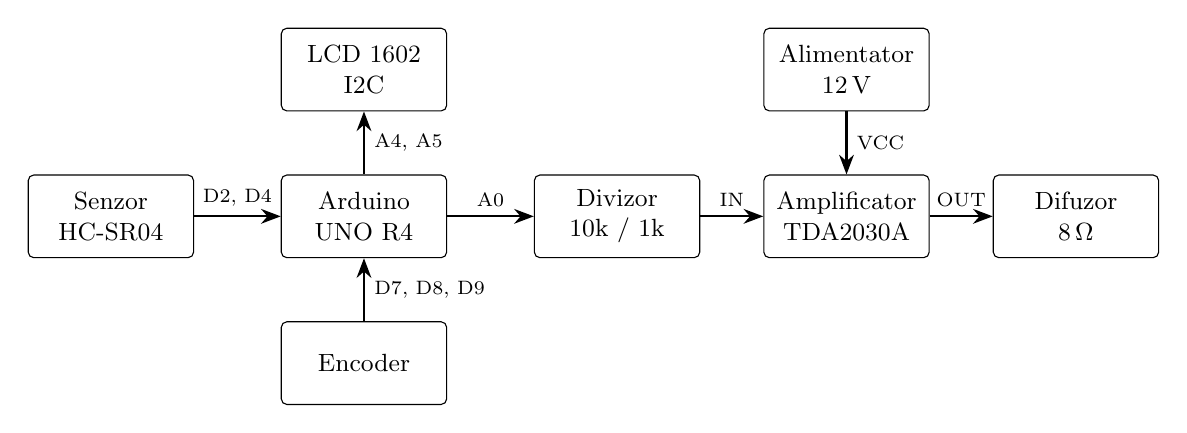
\begin{tikzpicture}[
  bloc/.style={draw, rounded corners=2pt, align=center, minimum height=1.05cm, minimum width=2.1cm, font=\small},
  sag/.style={-{Stealth[length=2.5mm]}, thick},
  eticheta/.style={font=\scriptsize},
  node distance=0.8cm]
  \node[bloc] (ard) {Arduino\\UNO R4};
  \node[bloc, left=1.1cm of ard] (senz) {Senzor\\HC-SR04};
  \node[bloc, above=of ard] (lcd) {LCD 1602\\I2C};
  \node[bloc, below=of ard] (enc) {Encoder};
  \node[bloc, right=1.1cm of ard] (div) {Divizor\\10k / 1k};
  \node[bloc, right=of div] (amp) {Amplificator\\TDA2030A};
  \node[bloc, right=of amp] (dif) {Difuzor\\8\,$\Omega$};
  \node[bloc, above=of amp] (alim) {Alimentator\\12\,V};
  \draw[sag] (senz) -- node[above, eticheta]{D2, D4} (ard);
  \draw[sag] (ard) -- node[right, eticheta]{A4, A5} (lcd);
  \draw[sag] (enc) -- node[right, eticheta]{D7, D8, D9} (ard);
  \draw[sag] (ard) -- node[above, eticheta]{A0} (div);
  \draw[sag] (div) -- node[above, eticheta]{IN} (amp);
  \draw[sag] (amp) -- node[above, eticheta]{OUT} (dif);
  \draw[sag] (alim) -- node[right, eticheta]{VCC} (amp);
\end{tikzpicture}
\caption{Schema bloc}
\end{figure}

%=====================================================================
\section{Obiective}

\begin{itemize}
  \item măsurarea distanței cu senzorul HC-SR04;
  \item transformarea distanței în frecvență, astfel încât fiecare centimetru să urce același interval muzical;
  \item generarea unei sinusoide cu DAC-ul plăcii, cu frecvență care variază continuu;
  \item legarea unui amplificator alimentat separat;
  \item folosirea unui LCD pe I2C și a unui encoder citit prin întrerupere.
\end{itemize}

%=====================================================================
\section{Noțiuni teoretice}

\textbf{Senzorul HC-SR04.} Trimite un puls de ultrasunete și măsoară cât durează până se întoarce ecoul; din acest timp se calculează distanța.

\textbf{Distanță și frecvență.} Frecvența crește exponențial când mâna se apropie, astfel încât fiecare centimetru urcă același interval muzical.

\textbf{Sinusoida.} Un timer cere de 48\,000 de ori pe secundă următorul punct al unei sinusoide, luat dintr-un tabel, și îl scrie în DAC. Frecvența se schimbă puțin la fiecare punct, deci variază continuu, fără trepte.

\textbf{Adaptarea nivelului.}
\[
  U_{\text{IN}} = U_{\text{DAC}} \cdot \frac{R_2}{R_1 + R_2} = U_{\text{DAC}} \cdot \frac{1\,\text{k}\Omega}{10\,\text{k}\Omega + 1\,\text{k}\Omega} \approx \frac{U_{\text{DAC}}}{11}
\]

%=====================================================================
\section{Componente necesare}
\label{sec:componente}

\begin{center}
\begin{tabularx}{\textwidth}{@{}l X@{}}
\toprule
\textbf{Componentă} & \textbf{Rol} \\
\midrule
Arduino UNO R4 & citește senzorul și encoderul, generează sunetul, comandă LCD-ul \\
Senzor ultrasonic HC-SR04 & măsoară distanța până la mână \\
Modul amplificator TDA2030A & amplifică semnalul pentru difuzor \\
Difuzor 8\,$\Omega$, 3\,W & produce sunetul \\
Alimentator 12\,V c.c. & alimentează amplificatorul \\
Rezistoare 10\,k$\Omega$ și 1\,k$\Omega$ & divizorul de semnal \\
Breadboard, fire Dupont & legăturile \\
LCD 1602 cu modul I2C & afișează nota, frecvența, volumul și modul \\
Encoder rotativ & volumul și schimbarea modului \\
Multimetru & verificarea alimentatorului \\
\bottomrule
\end{tabularx}
\end{center}

%=====================================================================
\section{Schema de conectare}

\begin{center}
\small
\begin{tabularx}{\textwidth}{@{}l l X@{}}
\toprule
\textbf{Componentă} & \textbf{Pin} & \textbf{Se leagă la} \\
\midrule
HC-SR04 & VCC / GND & 5V / GND Arduino \\
        & Trig / Echo & D4 / D2 \\
\midrule
LCD (modul I2C) & VCC / GND & 5V / GND Arduino \\
                & SDA / SCL & A4 / A5 \\
\midrule
Encoder & + / GND & 5V / GND Arduino \\
        & CLK / DT / SW & D8 / D9 / D7 \\
\midrule
Divizor & R1 = 10\,k$\Omega$ & între A0 și intrarea IN a amplificatorului \\
        & R2 = 1\,k$\Omega$ & între IN și GND \\
\midrule
TDA2030A & VCC & plusul alimentatorului de 12\,V \\
         & GND (primul) & GND Arduino \\
         & GND (al doilea) & minusul alimentatorului de 12\,V \\
         & clema OUT / GND & difuzorul \\
\bottomrule
\end{tabularx}
\end{center}

CLK-ul encoderului este pe D8 pentru că, pe UNO R4, D9 nu poate genera întreruperi. Pinii modulului TDA2030A se citesc după inscripțiile de pe spatele plăcii. Cei 12\,V ajung doar la pinul VCC al amplificatorului, niciodată la placa Arduino.

\begin{figure}[H]
\centering
\begin{minipage}[b]{0.47\textwidth}\centering
  \fisier{\linewidth}{tda2030a_spate.jpg}
  \caption{TDA2030A, spatele modulului}
\end{minipage}\hfill
\begin{minipage}[b]{0.47\textwidth}\centering
  \fisier{\linewidth}{tda2030a_fata.jpg}
  \caption{TDA2030A, văzut de sus}
\end{minipage}
\end{figure}

\begin{figure}[H]
\centering
\begin{minipage}[b]{0.47\textwidth}\centering
  \fisier{\linewidth}{montaj_complet.jpg}
  \caption{Montajul complet}
\end{minipage}\hfill
\begin{minipage}[b]{0.47\textwidth}\centering
  \fisier{\linewidth}{lcd_functionare.jpg}
  \caption{LCD-ul în timpul funcționării}
\end{minipage}
\end{figure}

\end{document}
